% #############################################################################
% This is Chapter 6
% !TEX root = ../main.tex
% #############################################################################
% Change the Name of the Chapter i the following line
\fancychapter{Integration of synthetic speech for data augmentation}
\label{chap:6}
\cleardoublepage

\section{Introduction}
% Challenge in children speech
As mentioned in Chapter \ref{chap:Chapter2}, the ongoing advancements in deep learning, coupled with the availability of extensive training datasets, have undeniably improved the ASR performances. However, despite these remarkable advancements, the recognition of children's speech remains a domain where performance lags behind that achieved for adult speech. Children's speech introduces distinct challenges owing to its inherent variability influenced by age, linguistic development, and articulatory differences. Therefore, there is a growing need acquiring a sufficiently diverse and extensive dataset for training children's ASR systems. 

However, practical constraints, including ethical considerations, privacy concerns, the high cost of data collection, the challenges posed by children's limited attention span and inconsistent adherence to prompts during reading tasks, hinder the creation of such datasets. In an effort to address this performance gap, researchers in \cite{asr-google} leveraged an in-house sizable dataset of children's speech, comparable in scale to an adult corpus, to train an ASR model. The outcomes showcased state-of-the-art performances, emphasising the potential of ASR systems to effectively learn from diverse and variable children's speech data when provided with a substantial amount of training data.

As an answer to the challenges of collecting real childen's speech data, an alternative strategy emerged, involving the generation of synthetic datasets using a Text-to-Speech (TTS) model. TTS offers a solution to bypass to the challenges associated with collecting and annotating real children's speech data. While some studies have explored the application of TTS for ASR, either through direct use of synthetic speech for training or as a form of data augmentation \cite{laptev2020you,fazel21_interspeech}, synthesising children's speech introduces a unique set of challenges. The inherent substandard and imprecise pronunciation in children's speech \cite{wang2021towards} poses an hurdle, raising concerns that the direct use of synthetic data may lead to a decrease in performance \cite{wang2021towards, hu2022synt++}.

% Our Approach
In this chapter, we introduce a novel technique known as ``Double-Way Adapter Tuning", or DWAT, to enhance ASR models specifically for children's speech, even in scenarios where imperfect data are employed as augmentation. Our approach involves the integration of additional Adapter modules into the existing ASR model during the fine-tuning process. As demonstrated in the preceding chapter \ref{chap:5}, Adapters have proven to be efficient in transferring knowledge for children's speech, thereby serving as a parameter-efficient means of knowledge transfer. But also as a novel way to reduce the gap between a source and target domain while preserving the source knowledge in the pre-trained model.
Building upon the efficiency of Adapters in the realm of children's speech, we hypothesise that these Adapters can be used to mitigate the domain mismatch between real and synthetic data. We accomplish this through a two-step training procedure in a similar way as the methodology proposed in \cite{fan2022draft}.

In the initial step, the Adapters are exclusively trained using synthetic data, while the pre-trained model remains frozen. This phase enables the Adapters to specialise in handling the nuances introduced by synthetic data. Subsequently, in the second step, we perform fine-tuning, involving both the trained Adapters and the entire model weights. During this fine-tuning process, a combination of synthetic and real data is given to the model. Notably, our approach introduces a crucial distinction between synthetic and real data throughout the fine-tuning process. Synthetic data traverses the Adapter layers, allowing the synthetic characteristics to be handle by the Adapters while  still contribute to the full model tunning, while real data bypasses these Adapters. We hypothesise that this meticulous differentiation could enables the effective use of imperfect synthetic data, ultimately leading to an enhancement in ASR performances.

In this chapter, our objective is to address the research questions: \textit{Is it possible to use children's synthetic speech to extend the amount of children's data? How can we control the quality and speakers’ variability?}

%In this chapter, we introduce a novel technique called "Adapter double-way fine-tuning" to enhance ASR models for children, even when using imperfect data augmentation. Our approach involves adding additional adapter layers to the existing ASR model during fine-tuning, similar to \cite{fan2022draft}. These adapter layers are customised to address the domain mismatch between real and synthetic data. We achieve this through a two-step training procedure. In the first step, the adapter layers are trained exclusively using synthetic data while keeping the pre-trained model frozen. In the second step, we fine-tune both the trained adapters and the entire model using a combination of synthetic and real data. Crucially, our approach differentiates between synthetic and real data during fine-tuning. Synthetic data passes through the adapter layers, while real data bypasses them. This approach enables the effective use of imperfect synthetic data to enhance ASR performance for children.


%\section{Related work}
\section{Enhancing ASR Performance through TTS Data Augmentation}
%TTS data augmentation
The progression of TTS systems, achieving human-like quality, presents a valuable avenue for effective TTS-based data augmentation in ASR. This approach, as exemplified in studies such as \cite{laptev2020you}, involves the generation of synthetic speech from text using TTS models. The synthetic speech is then combined with real speech during the training process, leading to notable performance enhancements. Importantly, this approach is not limited to well-resourced tasks and has demonstrated success even in low-resource scenarios, as illustrated in \cite{casanova2022asr}. However, despite its efficacy, TTS-based data augmentation offers only modest improvements, primarily owing to the persistent challenge of domain mismatch between synthetic and real speech, indeed, even with human-like quality, some generated utterances suffer artefacs or wrong modelisation. The inherent differences between the characteristics of synthetic and real speech limit the extent to which the benefits of TTS augmentation as ASR data augmentation. 
%The advancement of TTS systems, achieving human-like quality, enables effective TTS-based data augmentation in ASR. This approach, as shown in studies like \cite{ laptev2020you}, involves generating synthetic speech from text using TTS models, then combining it with real speech for training, resulting in performance enhancements. Notably, this approach is not limited to well-resourced tasks and has succeeded in low-resource scenarios, as demonstrated in \cite{casanova2022asr}. Nevertheless, TTS data augmentation offers only modest improvement due to the domain mismatch between synthetic and real speech. 
% To this end, \cite{9688218} proposed to use discrete representations based on VQ-wav2vec, allowing to mitigate the mismatch with real data and reducing speaker dependency.


In order to mitigate the mismatch with real data and to reduce speaker dependency,  the use of discrete intermediate representations both shared by the TTS and ASR systems instead of Mel-scale filterbanks, obtained with a VQ-wav2vec, has been proposed in \cite{9688218}. This approach has demonstrated promising results. However, it is essential to note that implementing such a strategy necessitates training both the ASR and TTS systems from scratch. This requirement may pose challenges, particularly in the context of low-resource ASR scenarios

% Children data selection
An alternative approach to address the domain mismatch between synthetic and real speech rely on data selection techniques, as proposed by \cite{wang2021towards}.  This approach focuses on selectively choosing high-quality synthetic speech data to mitigate the challenges associated with imperfect data augmentation. The data selection process ensures that only the most reliable and accurate synthetic speech samples are incorporated during the augmentation process. One advantageous aspect of this work is that it does not necessitate more complex training for the TTS or ASR system. Instead, it operates as an off-the-shelf selection on top of the TTS system. This characteristic underscores the practicality and ease of it integration into existing TTS systems.
In \cite{wang2021towards}, they demonstrated the effectiveness of employing i-vector speaker-embedding cosine similarity between reference and generated utterances as a metric for data selection. This metric was compared to other metrics such as error rate, acoustic posterior, and synthetic discriminator. 
%Another approach to mitigate the domain mismatch between synthetic and real speech is through the use of data selection techniques, as suggested by \cite{wang2021towards}. By selectively choosing high-quality synthetic speech data. This data selection process ensures that only the most reliable and accurate synthetic speech samples are used during data augmentation. The results presented in \cite{wang2021towards} demonstrate the effectiveness of employing i-vector speaker-embedding cosine similarity as a metric for data selection, compared to metrics like error rate, acoustic posterior, and synthetic discriminator.

% Synth++
More recently, \cite{hu2022synt++} introduced the Synth++ framework, which employs a similar data selection approach, called rejection sampling. This rejection sampling method relies on the output of a DNN, which is trained on a 5-dimensional features vector derived from a pre-trained ASR model. The goal of this DNN is to discriminate either the data is real or synthetic. To this end, the 5-dimensional features vector for each utterances encompass cross-entropy loss, CTC loss, WER, lengths of tokens in the predicted text and the length of tokens in the target text. In addition to rejection sampling, Synth++ introduces the use of separate batch normalisation for real and synthetic data. During the training process, when synthetic data is fed into the model, it undergoes distinct normalisation layers. The incorporation of this separated normalisation has been demonstrated to significantly reduce the mismatch between real and synthetic data during training, leading to notable improvements in WER scores.

% In Synth++ \cite{hu2022synt++}, an extension to the data selection technique is proposed, by incorporating separate batch normalization statistics for real and synthetic samples. While data selection handles artefacts and over/under-sampling, double batch normalization aims to further bridge the synthetic-real data gap during training. This approach uses rejection sampling based on a DNN's output. Where the DNN is trained on a 5-dimensional features vector derived from a pre-trained ASR model, including cross-entropy loss, CTC loss \cite{First_End2End}, word error rate (WER), lengths of tokens in prediction text, and length of tokens in target text, offering valuable insights into speech quality and characteristics.
% However, we find out that it may not be working. HERE?

\section{Closing the synthetic and real mismatch gap with Adapters}

\begin{figure*}
    \centering
    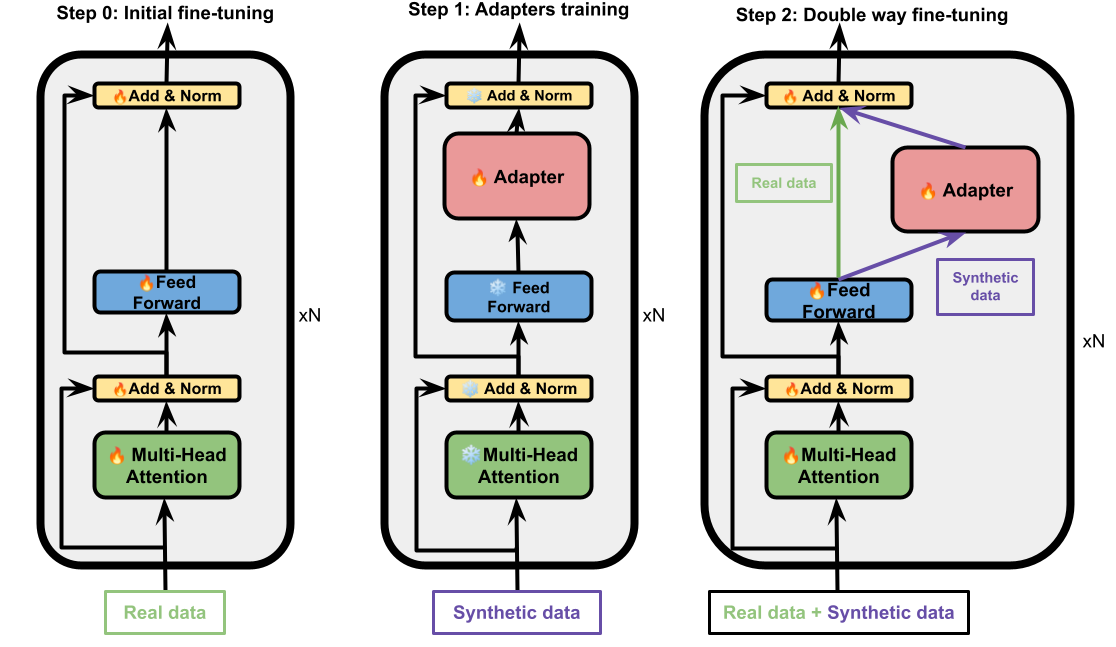
\includegraphics[width=\textwidth]{imgs/TTS_Transformer.png}
    \caption{Overview of ``Double way Adapter fine-tuning"  within th context of an Transformer model}
    \label{fig:overall}
\end{figure*}

The effectiveness of Adapters in the existing literature for both speech and NLP tasks has been well-documented \cite{pfeiffer, philip2020monolingual, mao-etal-2022-unipelt}. Additionally, the positive results detailed in Chapter \ref{chap:5}, where Adapter modules were proven effective for children's ASR, underscore their pivotal role in mitigating the mismatch between a source model and a target task. Proving that Adapters are capable of capturing task-relevant information, while the frozen pre-trained model retains valuable insights about the source task.

In alignment with these findings, \cite{fan2022draft} introduced the Domain Responsible Adaptation and Fine-Tuning framework (Draft) for children's ASR. The authors aimed to reduce the mismatch between adult and children speech data in SSL models by incorporating Adapters and an additional adaptation phase. Leading to improved performances.

Motivated by the successes of the Draft framework and Synth++, our approach integrates Adapter modules as a substitute for the separate normalisation layers present in the Synth++ framework. Furthermore, we incorporate the multiple-step adaptation and the use of Adapters from the Draft framework. Finally, we employed filtered synthetic data, implementing a speaker-embedding cosine similarity metric to retain synthetic utterances that exhibited high-quality generation as pproposed by previous work on data selection for TTS data augmentation. This combination forms a novel strategy to address the domain mismatch in ASR for children's speech, called ``Double-way Adapter tunning" (DWAT). 


Our primary goal is to inject external knowledge of synthetic children's speech into a pre-trained ASR model using Adapters. This approach allows us to preserve the real children's speech knowledge acquired during pre-training while separately modeling the synthetic characteristics within the Adapter modules. Therefore, Adapters serves as a bridge, that can effectively reducing the domain mismatch between real and synthetic speech data during the training of ASR models for children using a combination of real and synthetic data. 

In our DWAT  methodology, as illustrated in Figure \ref{fig:overall}, we introduce two additional steps following the standard ASR model training with children's data (Step 0).
% Step 1
Step 1 involves the standard training of Adapter modules, as explained in the previous chapter. While keeping the pre-trained ASR model parameters fixed, the Adapter weights are trained on the target data, here TTS utterances. These Adapter modules are strategically placed after the transformer layers' Feed-Forward Network (FFN) component. The goal is to learn a projection that aligns synthetic children's speech with real children's speech within each transformer layer. This approach allows the model to retain knowledge about children's speech, while the Adapters aim to capture the synthetic characteristics of the different TTS utterances. This step is crucial, as Adapter modules require this learning process. Without it, the subsequent fine-tuning in Step 2 could be more challenging and less effective.
%Step 1 entails the regular training Adapter modules, as presented in previous chapter. While keeping the pre-trained ASR model parameters fixed the Adpaters weights are being trained. These Adapter modules are placed after the transformer layers' FFN component, aiming to learn a projection that aligns synthetic children's speech with real children's speech within each transformer layers. By doing this, the model will still contains knowledge about children's speech while the Adapters should models the synthetic characteristics of the TTS utterances. This step is crucial as Adapter modules require this learning process. Without it, the subsequent fine-tuning in Step 2 could be more challenging and less effective.
%Step2
In Step 2, we fine-tune both the Adapters trained in Step 1 and the entire pre-trained ASR model using a mix of synthetic and real data. A pivotal aspect of our approach lies in how we handle data flow within the model. Real samples bypass the Adapter modules as they do not need further adjustments, directly passing through the original ASR model components. In contrast, synthetic data goes through the Adapters for necessary modifications to better align with real children's speech characteristics. This differential treatment of data optimises Adapter usage, potentially enhancing the overall performance of the ASR system.
%In Step 2, we fine-tune both the Adapters trained in Step 1 and the pre-trained ASR model using a mix of synthetic and real data. A crucial aspect of our approach is how we handle data flow within the model. Real samples bypass the adapter modules as they do not need further adjustments, directly passing through the original ASR model components. Synthetic data, on the other hand, goes through the Adapter for necessary modifications to align better with real children's speech characteristics. This differential treatment of data optimises adapter usage, potentially improving the ASR system's overall performance.
% Inference
During the inference phase, the Adapter modules become unnecessary and are discarded since the test data only contains real samples and the training is already complete. It is essential to note that Steps 1 and 2 can be iteratively repeated with newly generated synthetic data. However, it's important to highlight that this aspect is not thoroughly investigated in this work and serves as a subject for future research. The potential iterative repetition of these steps could provide insights into the adaptability and generalisation capabilities of the proposed Double-Way Adapter Tuning methodology.
%During inference, the Adapter modules become unnecessary and are discarded because the test data only contains real samples. It is important to mention that Steps 1 and 2 can be iteratively repeated with newly generated synthetic data, although this aspect is not investigated in this paper and is a subject for future research.


%Building on the successes observed with Adapters in the existing literature for speech and NLP tasks \cite{pfeiffer, philip2020monolingual, mao-etal-2022-unipelt}, and the results detailed in Chapter \ref{chap:5}, where Adapter modules were found to be effective for children's ASR, we propose leveraging Adapter modules to bridge the gap between real and synthetic speech data. 

%The motivation of our work is to expend on the achievements of the Draft framework and Synth++. Indeed, our approach use Adapters as a substitute for the double batch normalisation layers present in the Synth++ framework and use the multiple step adaptation with Adapters from Draft.

% Explain adapters
%Adapters were first introduced for natural language processing (NLP) tasks as a simpler alternative to full model fine-tuning \cite{houlsby}. They involve adding a small number of extra parameters to each layer of the transformer model. Unlike full fine-tuning, which modifies the entire model, adapters enable targeted adjustments within specific layers while keeping pre-trained parameters intact. These adapters typically follow a bottleneck architecture with down-projection and up-projection, as seen in Figure \ref{fig:overall}-b. The bottleneck architecture's purpose is to introduce non-linear transformations, enabling Adapters to capture task-specific features and learn task-specific modifications effectively.

%Since their proposal, adapters have demonstrated effectiveness in diverse NLP tasks, including language understanding and neural machine translation \cite{philip2020monolingual}. Additionally, there is a growing interest in applying adapters to automatic speech recognition. For instance, \cite{tomanek2021residual} explored adapters for atypical speech, focusing on pathological and accented speech.
% Draft
%In children's ASR, Adapters are employed within the Draft framework \cite{fan2022draft}. This approach inserts and trains Adapters at each block of a pre-trained self-supervised learning (SSL) model using an SSL loss. Subsequently, the entire model, including the Adapters, undergoes fine-tuning with ASR losses. By combining SSL pre-training, Adapters, and full fine-tuning, this approach uses the advantages of SSL, the adaptability of adapters, and task-specific fine-tuning to enhance the recognition accuracy of ASR systems for children's speech.

%\section{Method}


% Motivation
%Expanding on the achievements of the Draft Framework and Synth++, our approach utilizes Adapters as a substitute for the double batch normalization layer of the Synth++ framework. Our aim is to improve the performance of a pre-trained ASR model through data augmentation using synthetic data. In our methodology, we employed filtered synthetic data, implementing a speaker-embedding cosine similarity metric to retain synthetic utterances that exhibited high-quality generation. Our approach introduces two extra steps following the standard ASR model training (Step 0).%NEW
%Figure \ref{fig:overall}-a provides an overview of our proposed methodology.

% Step 1
%Step 1 entails training Adapter layers while keeping the ASR model parameters fixed. These Adapter layers are placed after the transformer layers' feed-forward component, aiming to learn a projection that aligns synthetic children's speech with real children's speech within the transformer layers. This step is crucial as Adapter layers require this learning process. Without it, the subsequent fine-tuning in Step 2 could be more challenging and less effective.

%Step2
%In Step 2, we fine-tune both the adapters from Step 1 and the pre-trained ASR model using a mix of synthetic and real data. A crucial aspect of our approach is how we handle data flow within the model. Real samples bypass the adapter layers as they don't need further adjustments, directly passing through the original ASR model components. Synthetic data, on the other hand, goes through the adapter layers for necessary modifications to align better with real children's speech characteristics. This differential treatment of data optimises adapter usage, potentially improving the ASR system's overall performance.

% Inference
%During inference, the Adapter layers become unnecessary and are discarded because the test data only contains real samples. It is important to mention that Steps 1 and 2 can be iteratively repeated with newly generated synthetic data, although this aspect is not investigated in this paper and is a subject for future research.
 
% Recap
In summary, our proposed approach use Adapter modules to enhance the performance of a pre-trained ASR model through the incorporation of synthetic data augmentation. This innovative methodology, known as DWAT introduces a two-step process involving the training of Adapter and subsequent fine-tuning with a mix of synthetic and real data in order to bridge the domain gap between real and synthetic children's speech.

%In summary, our approach uses adapter modules to improve the performance of a pre-trained ASR model through the integration of filtered synthetic data augmentation.




\section{Overview of the automatic speech recognition and text-to-speechs systems}
\label{section:SOA}
\subsection{Transformer architecture for ASR}
% Motivation children E2E
%The Transformer architecture, initially developed for tasks like machine translation \cite{Transformer}, was found to be highly effective and widely used in various domains, including computer vision \cite{VIT} and language understanding \cite{Bert}. In speech recognition, it takes acoustic features as input, processes them through an encoder to create high-level representations, and uses these for token prediction in a decoder. Training typically combines a sequence-to-sequence approach with a CTC loss \cite{CTC}.
%Recent studies, such as \cite{sri_end2end}, demonstrate that fine-tuning adult pre-trained Transformer-based models with children's speech data yield better results than traditional HMM-DNN based models, making the Transformer-based and End-to-end models a suitable choice for children's ASR.
In our experiments, we employed the SpeechBrain toolkit \cite{speechbrain} for the ASR component of our system, using a pre-trained Transformer model\footnote{https://huggingface.co/speechbrain/asr-transformer-transformerlm-librispeech}. This model has trained on the LibriSpeech dataset \cite{librispeech} and comprises 12 encoder layers and 6 decoder layers, each with a dimension of 512. It is noteworthy, that is model is different from the ones used in previous Chapters. A mix of sequence-to-sequence and CTC loss where used with respective weight of 0.7 and 0.3. Additionally, we integrated a Transformer language model trained on a 10 million-word transcriptions of Librispeech.

\subsection{Multi-speaker text-to-speech: YourTTS}

\begin{figure}
    \begin{center}
        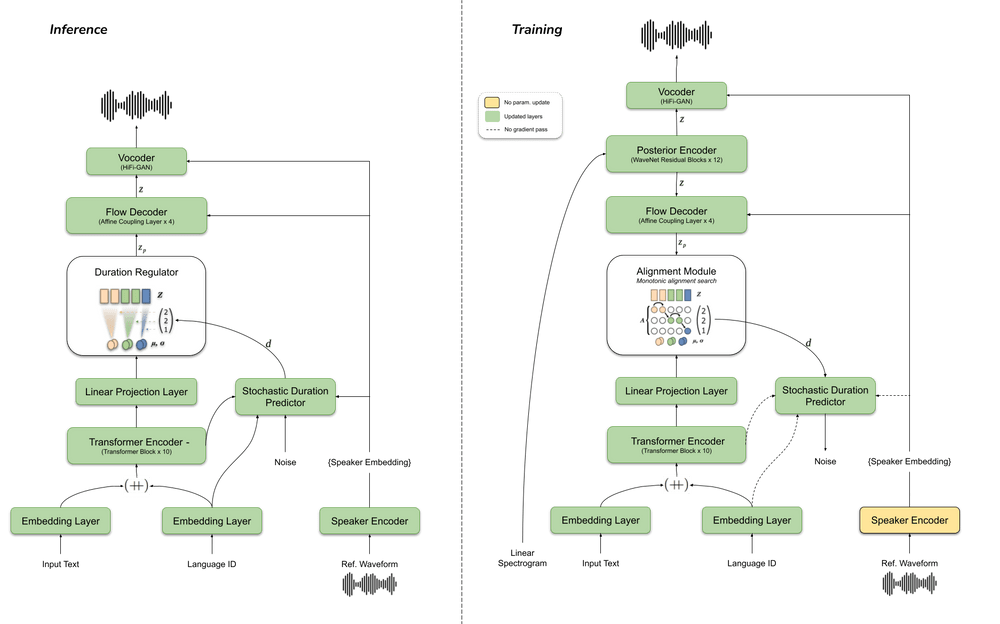
\includegraphics[scale=0.4]{imgs/yourtts.png}
        \caption{Architecture of the YourTTS model taken from \cite{casanova2022yourtts}}
        \label{fig:yourtts}
    \end{center}
\end{figure}

In this work as TTS component, we used the pre-trained YourTTS model\footnote{https://coqui.ai/blog/tts/yourtts-zero-shot-text-synthesis-low-resource-languages} proposed by \cite{casanova2022yourtts} based on the  Coqui toolkit. YourTTS is a zero-shot multi-speaker and multilingual TTS system that is built upon the Variational Inference with adversarial learning for end-to-end Text-to-Speech (VITS). It incorporates several novel modifications to enable zero-shot multi-speaker and multilingual synthesis. An overview of the YourTTS architecture is presented in Figure \ref{fig:yourtts}.
% General description of YourTTS
YourTTS featuring a 10-layer Transformer-based text encoder with 196 hidden channels. This encoder, adaptable for multilingual use, employs a 4-dimensional language embedding concatenated with the embedding of each input character. However, for the purpose of our experiment, the model use exclusively the English language. The decoder comprises four affine coupling layers \cite{45819}, each incorporating four WaveNet blocks \cite{45774} to ensure high-quality speech generation. The model also use the HifiGAN vocoder \cite{kong2020hifi}. Notably, YourTTS adopts an end-to-end approach, connecting the vocoder to the TTS model through a variational autoencoder (VAE) \cite{VAE}.

To enhance its capabilities as multi-speaker and zero-shot TTS system, YourTTS integrates a speaker encoder, specifically the H/ASP speaker encoder \cite{heo2020clova}, generating 512-dimensional speaker embeddings for each utterances. This speaker encoder models is compromising a CNN layers, followed by four Resnet layers \cite{targ2016resnet}, a attentive statistic pooling and a output linear layer. These embeddings serve as reference speakers for the model, enabling zero-shot multi-speaker capabilities. To give the model zero-shot multi-speaker generation capabilities, the authors conditioned all affine coupling layers of the flowbased decoder, the posterior encoder, and the vocoder on external speaker embeddings. Additionally, a speaker consistency loss (SCL) is added to the loss to further enhance the multi-speaker ability of the model. The SCL is formally expressed as follows:

\begin{equation}
    L_{SCL} = \frac{-\alpha}{n} \cdot \sum_{i}^{n} cos\_sim(\phi(g_i), \phi(h_i))
\end{equation}
where let $\phi(\cdot)$ is the function outputting the speaker embeddings, $cos\_sim$ is the cosine similarity function, $\alpha$ is a positive real number controlling the influence of the SCL in the final loss, $n$ is the batch size and $g$ and $h$ represent, respectively, the ground truth and the generated speaker audio.

The YourTTS model was trained using three languages: English with VCTK \cite{veaux2016superseded}, Brazilian Portuguese with TTS-Portuguese Corpus \cite{casanova2022tts}, and French with the French set of the M-AILABS dataset \cite{mailabs}. This training corpus totaled 229 hours of speech data and involved 115 speakers. For a more in-depth understanding of the YourTTS architecture and training process, detailed information can be found in the original paper \cite{casanova2022yourtts}.
% Architecture (specific to the model we used)
%YourTTS use a 10-layer Transformer-based text encoder with 196 hidden channels. It can be used in a multilingual fashion by using a 4-dimensional language embedding concatenated with the embedding of each input character, for the purpose of our experiment, the multi-lingual aspect was discarded to only keep the English language. The decoder has four affine coupling layers, each with four WaveNet blocks for high-quality speech generation. YourTTS uses an external H/ASP speaker encoder to generate 512-dimensional speaker embeddings for individual speakers, serving as reference speakers for the model. Additionally, YourTTS incorporates a HifiGAN vocoder \cite{kong2020hifi}. As YourTTS is an end-to-end model, the vocoder is connected to the TTS model using a variational autoencoder (VAE). For a comprehensive understanding of the YourTTS architecture and training, detailed information can be found in the original paper \cite{casanova2022yourtts}.


\section{Experimental setup}
\label{section:methods}

\subsection{Real speech corpus}
\begin{table}[h!]
\caption{My Science Tutor Children Speech Corpus statistics}

\begin{center}
\begin{tabular}{r|c|c|c}
\hline
 & Training & Validation     & Test   \\ \hline
\# of utterances & 60897   & 10044    & 4079  \\ 
\# of speakers & 566   & 79    & 91  \\ 
\# of hours & 113   & 18    & 13  \\ \hline
\end{tabular}
\label{tab:statistics}
\end{center}
\end{table}
In this study, we used the My Science Tutor (MyST) Children Speech Corpus, referred to as the "Real" set. This corpus contains around 400 hours of speech collected from 1,372 students in grades three to five. It comprises conversations with a virtual tutor spanning eight scientific domains. 
%To ensure equitable domain representation, the corpus has been partitioned, with each student's data in a single partition. 
Notably, only 45\% of the utterances in the corpus are transcribed. For our experiments, we filtered out utterances shorter than one second and longer than 30 seconds due to GPU memory constraints. Additional details on the filtered corpora are provided in Table \ref{tab:statistics}.

\subsection{Synthetic data}
% Finetune YourTTS with MyST train set
To address the potential performance gap caused by the YourTTS model being trained solely on adult data and never exposed to children's data, we initiated the process by fine-tuning the YourTTS model using the MyST training set. In this study, two TTS systems were developed, each with distinct parameter settings, to examine their respective performances and outputs quality under varying conditions. Two TTS systems, TTS$_1$ and TTS$_2$, were developed with distinct parameter settings. The first model, called TTS$_1$, underwent fine-tuning for 250 epochs, focusing without incorporating the speaker encoder SCL loss. In contrast, the second system, labelled TTS$_2$, was fine-tuned for 50 epochs, incorporating the speaker encoder SCL loss. This incorporation should improve the alignment between the generated speech and the reference speaker embedding provided to the model. These variations in training strategies enable a thorough examination of the model's performance and output quality under varying conditions,
%The first model, referred to as TTS$_1$, underwent fine-tuning for 250 epochs without including the speaker encoder loss. In contrast, the second system, labelled TTS$_2$, was fine-tuned for 50 epochs while incorporating the speaker encoder loss. This incorporation improved the alignment between the generated speech and the reference speaker embedding provided to the model.

% Use randomly selected speaker utterances from the training set, d-vector -> TTS
The first TTS model, TTS$_1$, was used to generate 300 hours of synthetic data referred to as \textit{Synth$_1$}. The second TTS model, TTS$_2$, was employed to generate a larger volume of synthetic data, up to 1,000 hours, denoted as \textit{Large Synth$_2 $}. To compare the performance of TTS$_1$ and TTS$_2$, a subset of 300 hours was extracted from the \textit{Large Synth$_2$} dataset, called \textit{Synth$_2$}. The full 1,000-hour set was exclusively used to evaluate the impact of different amounts of synthetic data, both with reduced and increased amount.

The speech synthesis process using the YourTTS model demands both a text transcription and a  speaker-embedding vector to generate a synthetic utterance. Therefore, to generate each utterances in both \textit{Synth$_1$} and \textit{Large Synth$_2$}, we randomly selected two utterances from the Myst training set, one designated for extracting the speaker embedding and the other exclusively used for its text transcription. The Myst training set, comprising a substantial 60,897 utterances, resulted in a vast pool of potential combinations, totaling 3,708,444,609. This extensive range of possibilities was strategically harnessed to introduce a deliberate mismatch between the selected speaker embeddings and their associated transcriptions. This intentional large range of possibilities served as a mechanism to infuse novel variability into the synthetic data, thereby introducing characteristics not present in the original real corpus.

%In both \textit{Synth$_1$} and \textit{Synth$_2$}, where generated by randomly selected d-vectors and text transcriptions from the MyST training set. Notably, the selected d-vectors did not match the associated transcriptions to introduce variability into the synthetic data.
% Use a randomly selected text transcription in order to fit the transcription style of MyST, "UM" for hesitations
The decision to use MyST transcriptions for generating synthetic data was driven by the aim to expose the TTS model to the unique transcription style present in the MyST dataset. This style encompasses elements such as "UM" hesitations. By adopting this strategy, we intended to enhance the model's ability to learn and reproduce the specific transcription characteristics of the MyST data.
%Our choice of using MyST transcriptions to generate synthetic data, was motivated by exposing the TTS model to the unique transcription style of the Myst dataset, including elements like "UM" hesitations. This approach helps the model learn and reproduce the specific transcription characteristics of the MyST data.

To ensure the quality of the synthetic utterances in \textit{Synth$_1$} and \textit{Large Synth$_2$}, we extended the approach proposed by \cite{wang2021towards}, which involves using cosine similarity between the speaker embeddings of the reference and synthetic utterances as a data selection criterion. However, instead of using i-vector speaker embeddings, we opted for an x-vector approach and employed a different speaker embedding extractor than the one used by the YourTTS model (to prevent conflicts with the SCL loss). Specifically, we used a pre-trained x-vector extractor trained on VoxCeleb\footnote{https://huggingface.co/speechbrain/spkrec-ecapa-voxceleb}. During the generation process, we applied a cosine similarity threshold of 0.75 to discard all poorly generated synthetic utterances. While exploring data selection mechanisms, we considered the rejection sampling method suggested by Synth++ \cite{hu2022synt++} but found it unsatisfactory, ultimately opting for speaker-embedding similarity as the selection criterion. To comprehensively evaluate the impact of this data selection, we also created \textit{Unfiltered Synth$_1$} and \textit{Unfiltered Synth$_2$}, two 300-hour corpora of synthetic data generated without using speaker embedding data selection, created with TTS$_1$ and TTS$_2$, respectively.
%To assess the filtering effect, we generated an extra 300-hour set for both \textit{Synth$_1$} and \textit{Synth$_2$} without using speaker embedding data selection. Our data selection method relied on cosine similarity using x-vectors from a pre-trained x-vector extractor\footnote{https://huggingface.co/speechbrain/spkrec-ecapa-voxceleb}. We applied a cosine similarity threshold of 0.75 to discard bad synthetic utterances. We also explored the data selection mechanism suggested by \cite{hu2022synt++} but found it unsatisfactory, opting instead for speaker-embedding similarity as the selection criterion.

\subsection{Experiments}
We conducted a comprehensive evaluation of our DWAT approach through a series of experiments, comparing it with existing methods. We started the process with baseline models, fine-tuning an pre-trained adult model to children's speech using \textit{Real} data for 20 and 25 epochs (referencing step 0 in Figure \ref{fig:overall}). Subsequently, we evaluated the performance of TTS models using only \textit{Synth$_1$} and \textit{Synth$_2$} data. To understand the impact of data filtering, we compared these models trained on filtered data with the unfiltered versions \textit{Unfiltered Synth$_1$} and \textit{Unfiltered Synth$_2$}. Additionally, we considered the combination of these synthetic datasets with \textit{Real} data. These models underwent training for 20 epochs.

We also explored the application of double-way normalisation, inspired by Synth++ \cite{hu2022synt++}. In one scenario, we fine-tuned the adult model for 20 epochs using a mix of filtered synthetic and real data with double-way normalisation (\textit{Norm double-way from adult} in Table \ref{tab:res}). In another scenario, we trained the double-way normalisation model for 5 epochs with the baseline model as initialisation, referred to as \textit{Norm double-way from children}.

Finally, we implemented our \textit{DWAT} approach, training the models for 5 epochs with the baseline model as initialisation. Various hyper-parameter configurations will be explored in section \ref{section:exp_DWAT}.

%We evaluated our Adapter double-way fine-tuning approach in a series of experiments, comparing it to existing methods. We started with baseline models fine-tuning an adult model to children's speech using real data for 20 and 25 epochs (step 0 in Figure \ref{fig:overall}-a).
%Next, we assessed the TTS models' performances using only \textit{Synth$_1$} and \textit{Synth$_2$} data. We also explored data filtering's impact by comparing models trained on filtered and unfiltered versions of \textit{Synth$_1$} and \textit{Synth$_2$}, along with their combination with \textit{Real} data. These models were trained for 20 epochs.
%We also explored double-way normalization inspired by Synt++. In one scenario, we fine-tuned the adult model for 20 epochs using a mix of filtered synthetic and real data with double-way normalization (\textit{Norm double-way from adult} in Table \ref{tab:res}). In another scenario, we trained the double-way normalization model for 5 epochs with the baseline model as initialization, referred to as \textit{Norm double-way from children}.
%Finally, we implemented our \textit{Adapter double-way} approach, training the models for 5 epochs with the baseline model as initialisation. Different hyper-parameter configurations will be explored in section \ref{section:exp}.
\section{Results and discussion}
\label{section:exp_DWAT}

\subsection{Comparison with existing approaches}

\begin{table}[t]
\centering
\begin{tabular}{ccc}
\hline
 Method & TTS$_1$ & TTS$_2$  \\ \hline
\multicolumn{1}{l}{\textit{Real (20 epochs)}} & \multicolumn{2}{c}{12.99\%}\\ 
\multicolumn{1}{l}{\textit{Real (25 epochs)}} & \multicolumn{2}{c}{13.15\%}\\ \hline
\multicolumn{1}{l}{\textit{Real} + Unfiltered \textit{Synth}}  &   13.41\%  & 13.24\% \\ 
\multicolumn{1}{l}{\textit{Real} + \textit{Synth} \cite{wang2021towards}} & 13.09\% & 12.98\% \\
\multicolumn{1}{l}{\textit{Synth} alone}    & 40.58\%  & 40.21\%  \\
\multicolumn{1}{l}{Two step adaptation}    & 13.49\%  & 13.46\%  \\
\hline
\multicolumn{1}{l}{Norm double-way (from adult)} & 12.89\% & 13.04\% \\ 
\multicolumn{1}{l}{Norm double-way (from children)} & 13.56\% & 13.87\% \\ \hline
\multicolumn{1}{l}{DWAT (Ours)} &\textbf{ 12.42\%} & \textbf{12.31\%} \\ \hline
\end{tabular}

\caption{Results of the different approaches (in WER).}
\label{tab:res_DWAT}
\end{table}

% Baseline
Table \ref{tab:res_DWAT} present the results of the various approaches. The baseline models, obtained by fine-tuning an adult model on children's speech using \textit{Real} data, achieved a WER score of 12.99\%. However, extending the training to 25 epochs resulted in an overfitting and a subsequent reduction in performance score with 13.15\% WER.
Moving to the impact of incorporating unfiltered synthetic data, denoted as \textit{Unfiltered Synth$_1$} and \textit{Unfiltered Synth$_2$}, as opposed to their filtered counterparts \textit{Synth$_1$} and \textit{Synth$_2$}, in conjunction with \textit{Real}. We observed that the inclusion of filtering presented a notable 2\% enhancement in WER when compared to the unfiltered counterparts. However, relying solely on filtered TTS speech (\textit{Synth} alone) without any \textit{Real} data, resulting in a substantial 40\% WER on the \textit{Real} test set for both TTS$_1$ and TTS$_2$. This discrepancy underscored the considerable domain mismatch between real and synthetic data, signaling the imperative need for further approaches to mitigate this gap.
Furthermore, we delved into a two-step adaptation process where we initially fine-tuned the adult model using only \textit{Synth} data, followed by a subsequent fine-tuning with \textit{Real} data. However, the results indicated a slight decrease in performance in both cases, with WER scores of 13.49\% and 13.46\%, respectively. This decline could be attributed to the gap between the characteristics of TTS data which may be bigger than the original adult data.

%Moving to the impact of unfiltered synthetic data \textit{Unfiltered Synth$_1$} and \textit{Unfiltered Synth$_2$} compared to their filtered \textit{Synth$_1$} and \textit{Synth$_2$} when concatenated with \textit{Real} data., we observed that the introduction of filtering led to a 2\% improvement in WER compared to the unfiltered counterparts. Yet, a notable observation is when solely relying on filtered TTS speech (\textit{Synth} alone), yielding a considerable 40\% WER on the \textit{Real} test set. This discrepancy underscored the substantial domain mismatch between real and synthetic data and the need of further approach to reduce it.

%The results of the various approaches are summarised in Table \ref{tab:res_DWAT}. Our baseline models achieved a WER score of 12.99\%. Training for 25 epochs led to over-fitting and a decrease in performance.
%Filtered and TTS alone
%Filtered \textit{Synth$_1$} and \textit{Synth$_2$} data improved WER by 2\% compared to unfiltered data, but using only filtered TTS speech (\textit{Synth} alone) resulted in a significant 40\% WER on the \textit{Real} test set, highlighting the domain mismatch between real and synthetic.
% Double-norm 
During our experiments, the use of double batch normalisation proved ineffective in enhancing the baseline model's performance. Instead, it led to a 5\% relative decrease in WER performance when evaluated with the baseline model as initialisation (from children). When training from the adult model, the results were consistent  with the baseline models, with no observed improvement. These results underscore the limitations of double batch normalisation in addressing the domain mismatch between real and synthetic speech data within a Transformer model. This highlights the importance of exploring alternative strategies to effectively bridge the gap.
%Our experiments found that double batch normalization did not improve the baseline model's performance and even led to a 5\% relative decrease in WER  performance when evaluated with the baseline model as initialisation. This highlights the need for alternative methods to address the domain mismatch between real and synthetic speech data.
% Adapter Double-way
Our proposed DWAT approach, initiated with the baseline model (step 0 in Figure \ref{fig:overall}), emerged as the most effective among all methods examined. It demonstrated a notable 4\% and 5\% relative improvement in WER over the baseline when evaluated on \textit{Synth$_1$} and \textit{Synth$_2$} respectively. This outcome highlights the efficacy of our approach compared to longer training on the \textit{Real} set, showcasing its potential in mitigating the challenges posed by domain mismatch in the context of Automatic Speech Recognition systems.
%Our double-way adapter fine-tuning approach, initialised with the baseline model (step 0 in Figure \ref{fig:overall}), outperformed all other methods. It achieved a 4\% and 5\% relative WER improvement over the baseline on \textit{Synth$_1$} and \textit{Synth$_2$} respectively, demonstrating the effectiveness of our approach compared to longer training on the \textit{Real} set.

% TTS robustness
%In conclusion, the experiments reveal that both double-way adapters, trained using data augmentation from \textit{Synth$_1$} and \textit{Synth$_2$}, outperformed the baseline and previous works. These results demonstrate the robustness of our approach, showcasing its effectiveness across different TTS configurations.

\subsection{Influence of synthetic number of hours}
\begin{table}[t]
\centering
\begin{tabular}{cc}
\hline
 Amount of TTS data & WER $\downarrow$   \\ \hline
\multicolumn{1}{c}{0h} & 12.99\% \\ \hline
\multicolumn{1}{c}{10h}  &   12.73\%   \\ 
\multicolumn{1}{c}{50h}    & 12.54\%   \\ 
\multicolumn{1}{c}{100h} & 12.49\%  \\ 
\multicolumn{1}{c}{300h} & \textbf{12.31\%}  \\ 
\multicolumn{1}{c}{600h} & 12.57\%  \\ 
\multicolumn{1}{c}{1000h} & 13.14\%  \\ \hline

\end{tabular}

\caption{Results of the different number of hours influence in our DWAT approach with \textit{Large Synth$_2$} data}
\label{tab:hours}
\end{table}

%Time experiments
Given the potential of our approach to generate a theoretically "infinite" amount of TTS data, our primary objective is to conduct a comprehensive exploration of the impact of varying data quantities on the efficacy of the DWAT approach. To achieve this, we assess the influence of different quantities of synthetic data from \textit{Large Synth$_2$}, as detailed in Table \ref{tab:hours}.
The findings from our investigation reveal that utilising a small quantity of synthesised speech, ranging from 10 to 50 hours, results in limited improvements in ASR performance. Conversely, an excessive volume of TTS data, spanning from 600 to 1,000 hours, has the potential to introduce undesirable noise into the system. Consequently, achieving an optimal equilibrium, typically within the range of 100 to 300 hours, becomes crucial. This balance aims to enhance robustness in ASR performance while concurrently preventing the introduction of excessive noise, thereby maximising the effectiveness of the DWAT approach.
%Table \ref{tab:hours} summarizes the impact of varying amounts of synthetic data from \textit{Synth$_2$} on our adapter double-way approach. Using a small amount of synthesized speech (10 to 50 hours) yields limited ASR performance improvement. While excessive TTS data (600 to 1,000 hours) can introduce noise. Thus, it's crucial to use an appropriate amount (100 to 300 hours) to balance between robustness and avoiding noise introduction.
\subsection{Impact of DWAT different hyper-parameters}
\label{sec:hyperparameter}
\begin{table}[t]
\centering
\begin{tabular}{cccc}
\hline
 Location &  Bottleneck size &  5 epochs &  20 epochs     \\ \hline
\multicolumn{1}{c}{Encoder} & 64 & 12.58\% & 12.24\% \\ 
\multicolumn{1}{c}{Encoder} & 128 &  12.31\% & 12.45\%  \\ 
\multicolumn{1}{c}{Encoder} & 256  & \textbf{12.25\%} & 12.32\%  \\ 
\multicolumn{1}{c}{Encoder} & 1024 & 12.42\% & \textbf{12.22\%} \\ 
\multicolumn{1}{c}{Encoder} & 2048 & 12.57\% & 12.47\% \\ \hline
\multicolumn{1}{c}{Encoder-Decoder} & 128 & 12.45\% & 12.48\% \\ \hline
\multicolumn{1}{c}{Skip step 0} & 256 & 12.30\% & - \\ 
\multicolumn{1}{c}{Skip step 0 and 1} & 256 & 13.28\% & - \\ \hline

\end{tabular}

\caption{Results of the different configurations of Adapter double-way approach on 300h of \textit{Synth$_2$}}
\label{tab:config}
\end{table}
To thoroughly evaluate the robustness of our approach, we conducted experiments with the DWAT in various configurations. This comprehensive analysis involved exploring different Adapters's bottleneck sizes, ranging from 64 to 2048, varying the number of training epochs (5 and 20), investigating the integration of Adapters in the decoder of the transformer model, and performing an ablation study by skipping step 0 and both step 0 and 1 in the DWAT process.
%To assess the robustness of our approach, we assessed the Double-way adapter in diverse configurations. This involved experimenting with different bottleneck sizes (ranging from 64 to 2048), varying the number of training epochs (5 and 20), exploring the use of Adapters in the decoder of the transformer model, and conducting an ablation study by skipping step 0 and step 0 and 1.

% Best config
The summarised results in Table \ref{tab:config} provide insights into the optimal configuration, revealing that the most effective setup uses Adapters with a size of 1024 in the encoder only, coupled with 20 training epochs. This configuration resulted in a remarkable 6\% relative WER reduction compared to the baseline. Notably, all configurations demonstrated superior performance to the baseline, underscoring the overall effectiveness of our DWAT approach.
%Table \ref{tab:config} summarizes the results, highlighting that the optimal configuration uses adapters with a size of 1024 in the encoder only, coupled with 20 training epochs, resulting in a  6\% relative WER reduction when compared to the baseline. Importantly, all configurations demonstrated superior performance to the baseline, underscoring the effectiveness of our approach.

% Other results
Our observations indicate that extended training periods were particularly advantageous for larger Adapter bottleneck sizes, demonstrating no signs of overfitting. Moreover, the integration of Adapters into the decoder did not lead to a significant improvement in results. This outcome can be attributed to the higher acoustic variability and the fact that the same transcriptions from the Myst dataset were used for synthetic speech utterances. Lastly, skipping step 0 (pre-training) did not result in a significant degradation in performance. However, when both step 0 and step 1 (pre-training and Adapter pre-training) were skipped, performance degradation occurred, underscoring the critical role of Adapter pre-training phase (step 1) in achieving good performances.
%Our findings suggest that extended training periods were beneficial for larger Adapter bottleneck sizes, without indications of overfitting. Moreover, adding Adapters to the decoder did not significantly improve results. Finally, skipping step 0 (pre-training) did not significantly degrade results, but skipping both step 0 and step 1 (pre-training and Adapter pre-training) led to performance degradation, indicating the importance of Adapter pre-training for improved performance.

\subsection{Extension DWAT to the Conformer architecture}
\begin{figure}
    \centering
    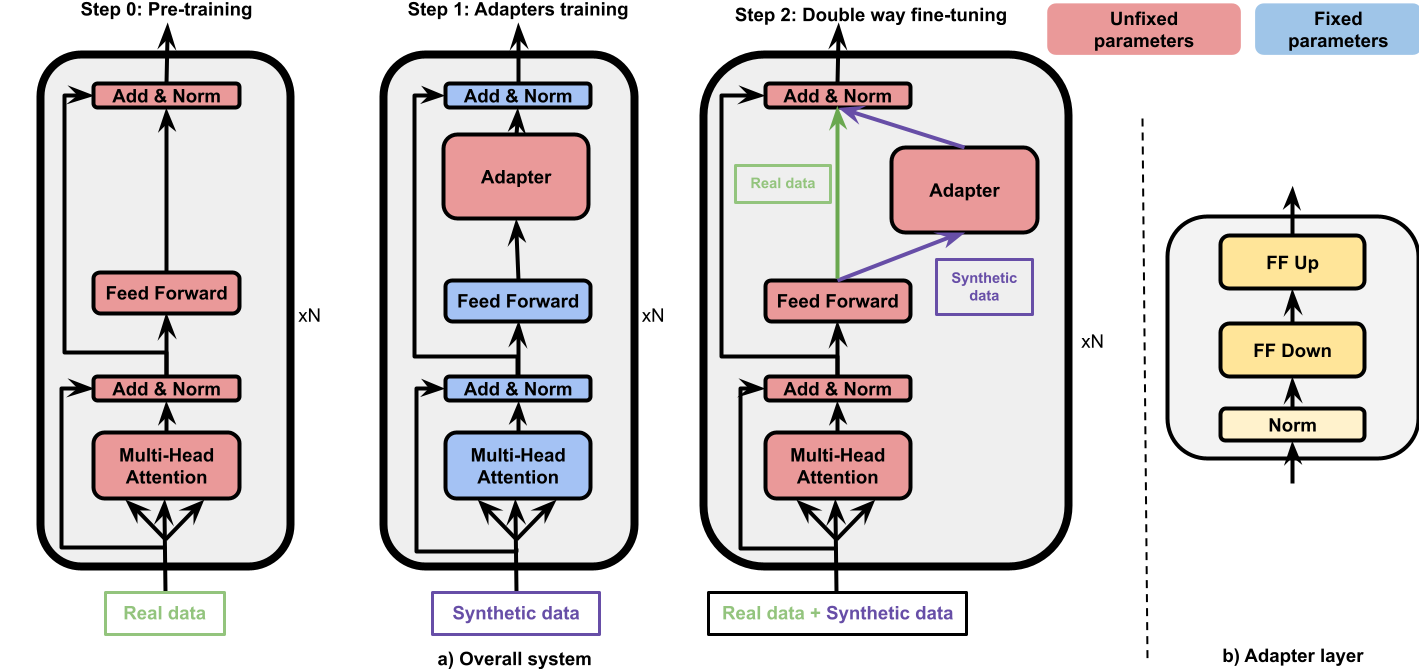
\includegraphics[width=\textwidth]{imgs/Overall_system.png}
    \caption{Overview of ``Double way Adapter fine-tuning"  within th context of an Conformer architecture}
    \label{fig:tts_conformer}
\end{figure}
Building upon the favorable results observed in previous chapters, which indicated that the Conformer model outperformed the regular Transformer for ASR tasks, the effectiveness of Adapters in Conformer and  considering that Synth++ \cite{hu2022synt++} was originally designed for the Conformer architecture, we decided to evaluate our DWAT within the Conformer architecture. Given that the TPA configuration of Adapters proved to be the most effective, we chose to implement it in our DWAT for the Conformer architecture. The DWAT with TPA is illustrated in Figure \ref{fig:tts_conformer}.

In this experiment, we employed the same pre-trained adult Conformer model used in previous chapters. This model comprises 12 layers of Conformer layers for the encoder, followed by 6 Transformer layers for the decoder, all with a hidden dimension of 512. The language model used is consistent with the experiments conducted with the Transformer model in the previous sections. Motivated by the insights gained from the exploration of hyperparameters in section \ref{sec:hyperparameter}, we opted for Adapters of size 512 in the Encoder only, using the TPA configuration. In term of training, Step 0 and step 1 were trained for 30 epochs while step 2 only used 10 epochs. 

\begin{table}[h]
    \centering
    \begin{tabular}{lr}
        \toprule
        Method & WER Score $\downarrow$ \\
        \midrule
        Adult model & 21.75\% \\
        \textit{Real} only & 12.28\% \\ \hline
        \textit{Unfiltered Synth$_2$} & 37.85\% \\
        \textit{Unfiltered Synth$_2$} + \textit{Real} & 12.30\% \\ 
        \textit{Synth$_2$} alone & 31.72\% \\
        \textit{Synth$_2$}+ \textit{Real} & 12.02\% \\ 
        Two step adaptation & 12.51\% \\ \hline
        Synth++ (norm double way) & 11.80\% \\
        DWAT & \textbf{11.64\%} \\
        \bottomrule
    \end{tabular}
    \caption{Scores for the different methods within the Conformer architecture}
    \label{tab:DWAT_conformer}
\end{table}

The results obtained from the extension of DWAT experiments using the Conformer architecture are presented in Table \ref{tab:DWAT_conformer}. The frozen adult model, referred as the Adult model, achieved a WER score of 21.75\%. When considering only real data (Real only), the WER score improved significantly to 12.28\%. Which is already outperforming the best results of the Transformer.

When using unfiltered synthetic data alone (\textit{Unfiltered Synth$_2$}) method, it resuted in a higher WER score of 37.85\%, showcasing, once again, the mismatch between synthetic and real data. However, when combined with real data (\textit{Unfiltered Synth$_2$} + \textit{Real}), the result are close to the real baseline with a WER score of 12.30\%. Similarly, using the filterd \textit{Synth$_2$} alone resulted in a WER score of 31.72\%, but when combined with real data (\textit{Synth$_2$} + \textit{Real}), the WER score decreased significantly to 12.02\%. This differ from the results observed in the Transformer architecture, as data filtering improved the WER score compared to the baseline.
Similarly to the Transformer, the two-step adaptation method yielded a WER score of 12.51\%. 

Further insights into the performance of the more sophisticated methods are provided in the context of the Conformer architecture. Specifically, the Synth++ method, which incorporates separated batch normalisation within each Convolution module for TTS data, achieved a WER score of 11.80\%. This contrasts with the results observed in the Transformer experiment, highlighting the efficiency of this approach specifically within Conformer models. In the other hand, the DWAT method consistently outperformed all other methods, showcasing a remarkable WER score of 11.64\%. These findings emphasise the effectiveness of both the Synth++ and DWAT methods in enhancing the Conformer architecture's performance on the given task.

It is important to highlight that while both Synth++ and DWAT demonstrate efficacy within the Conformer setup, the DWAT approach consistently outperforms other methods in both Transformer and Conformer configurations. This consistent superiority underscores the relevance and robustness of the DWAT approach in improving the overall performance of the models across different architectures.

In summary, the experimental results demonstrate the effectiveness of leveraging synthetic data, real data, and advanced adaptation methods within the Conformer architecture. The DWAT method, in particular, stands out as the most successful approach in minimising the WER.


\section{Summary and discussion}
\label{section:conclusions_tts}

In this chapter, we aimed to answer to the following research questions: \textit{Is it possible to use children's synthetic speech to extend the amount of children's data? How can we control the quality and speakers’ variability?}

% Summary 
We provide positive responses to both research questions through the introduction our a novel methodology: the Double way Adapter Transfer procedure, which combine Adapters and synthetic data augmentation for children's speech recognition. Our two-phase training strategy consist of the initial training of Adapter modules using synthetic data, followed by the fine-tuning of Adapters and the entire model weights using a hybrid dataset comprising both synthetic and real data. This distinctive dual-pathway approach resulted in notable improvement over baseline and previous techniques across various configurations. Importantly, our approach demonstrated robustness across different ASR architectures, TTS model fine-tuning parameters, Adapter sizes, number of epochs, and varying amounts of synthetic data. Furthermore, our study showcases the controllability of TTS output quality without necessitating direct modifications of the TTS model. This filtering process, performed before applying the DWAT, is achieved through the use of pre-trained x-vectors speaker embeddings and cosine similarity metrics between reference and generated utterances. This approach, improved from previous work which only used i-vectors \cite{wang2021towards}, allows the use of synthetic data which align more closely with desired characteristics of real children's speech, contributing to a more controlled augmentation process.

% Discussion
The promising performances observed with the DWAT pave the way for future research avenues. One potential avenue involves adopting an iterative methodology, dynamically incorporating newly generated TTS data while adjusting the proportion of real data. This iterative fine-tuning approach could potentially provide further insights into the interaction between synthetic and real data, offering opportunities to refine and optimise the training process for improved children's ASR models.
Another avenue for exploration could extend the DWAT framework to domains beyond the synthetic and real speech data. Investigating the adaptability and effectiveness of DWAT in diverse domains. In the context of children's ASR, the adult and children's speech domain could be an interesting first step towards this direction.
Furthermore, considering the rapidly evolving landscape of PETL approaches, the exploration of new modules as replacements for Adapters represents an new research direction. To this end, in the upcoming chapter, we delve into a comprehensive evaluation of various PETL alternatives, aiming to identify novel strategies for enhancing children's ASR systems.